\documentclass{fisattraining}
\title{My report Title}
\team{Tania Susan Sajeev}
\author{My Name}
\begin{document}
\maketitle
\makecert

\newpage
\pagenumbering{roman}
\setcounter{page}{1}
\newgeometry{top=4cm,bottom=0.1cm}
\thispagestyle{plain}
\renewcommand\abstractname{Company Profile}
\begin{abstract}
\vspace{5cm}
WiSilica is a provider of a leading IOT platform that securely bridges objects, locations, people and cloud. WiSilica enables smart environments where IoT connected devices understand contextual elements, such as proximity and de-centralized control, putting the intelligence into the devices themselves, via local preconfigured networks. A true smart environment where customers can connect smart homes, buildings, lighting, sensors and wearables into intelligent devices managed by mobile apps and the cloud. WiSilica is the only company that enables a complete smart environment through its Bluetooth low-energy (BLE) based mesh networking IoT platform. WiSilica believes that devices themselves need to “understand the human.” Smart environments and devices need to learn when to suggest and respond to prompts, as well as figuring out how to allow the user to opt into certain actions, rather than having prompts and triggers configured in advance. WiSilica’s WiSe Connect platform is a secure, scalable, simplified IOT platform that provides superior ROI, faster time to market, and strong customer support. Security: WiSilica’s security starts at their h/w reference design and device identity, and extends to secure communication between devices and devices to cloud, data protection, enterprise level authentication and authorization. Scalable: Provides scalable infrastructure that supports for variety of device types including third party vendors and protocols and cloud. Simplified: Provides ease of installation and operation to end users. Superior ROI: Low cost both upfront and growth, and reduces risk by being able to tryout devices without requiring bridges or cloud. Time to market: WiSilica’s generic h/w modules, firmware, app and cloud open API are easily adoptable. Customer Support: WiSilica’s professional services can help quickly integrate h/w modules, create apps and deploy cloud as well as provide a turnkey solution from design to deployment.

Website
http://www.wisilica.com

Headquarters
Laguna Hills, CA

Physical address per location :
Adam Square, Pallikara Road,, Athani,Kusumagiri P O, Kakkanad, Kochi, Kerala 682030, India

Year Founded
2013
Company Type
Privately Held

Size
51-200 employees

Specialties
Bluetooth 4.0 Low Energy Mesh, Real Time Tracking Solution (RTLS), App &amp; Cloud GUI design for Android and IOS, SaaS and PaaS for all WiSilica Bluetooth Solutions, Network Lighting Control Solutions, Bluetooth enablement , Bluetooth SIG Member, Bluetooth 5.0 Product Development, OEM &amp; ODM Product Development, Tunable White Controls, Agriculture Lighting Controls, Energy Management Platform, Bluetooth Snsor Technology, BLE Asset Tracking, Bluetooth Patient Tracking

\end{abstract}


\newpage
\renewcommand\abstractname{ACKNOWLEDGMENT}
\thispagestyle{plain}
\begin{abstract}
\vspace{5cm}
It is indeed a great pleasure for me to present this internship training report on IOT as a part of the curriculum of the Bachelor of Technology (Computer Science Engineering) degree.
I take this golden opportunity to thank all my mentors at WISILICA PVT. Who with their support and venerated guidance made this training a real success. I express my sincere thanks to officers of WISILICA PVT. Who in spite of their busy schedule have lent their precious time for helping out me to understand various systems used in WISILICA PVT.
I will be failing in my duty if I am not mentioning the technical demonstrations as given by the reverent staff of WISILICA PVT. Getting training at suck an organization is an exquisite learning experience that made a mark at the profoundest part of my mind.

\vspace{1cm}
\begin{flushright}
Tania Susan Sajeev
\end{flushright}
\end{abstract}
\newpage

\restoregeometry
\tableofcontents
\newpage

\cleardoublepage
\addcontentsline{toc}{chapter}{\listfigurename}
\listoffigures
\newpage

\cleardoublepage
\addcontentsline{toc}{chapter}{\listtablename}
\listoftables
\newpage



\chapter{Technology}
\pagenumbering{arabic}
\setcounter{page}{1}
\renewcommand{\baselinestretch}{1.50}
\section{Introduction}
The mathematical roots of the idea of fractals have been traced through a formal path of published works, starting in the 17th century with notions of recursion, then moving through increasingly rigorous mathematical treatment of the concept to the study of continuous but not differentiable functions in the 19th century, and on to the coining of the word fractal in the 20th century with a subsequent burgeoning of interest in fractals and computer-based modelling in the 21st century.
\begin{figure}[h!]
\begin{center}
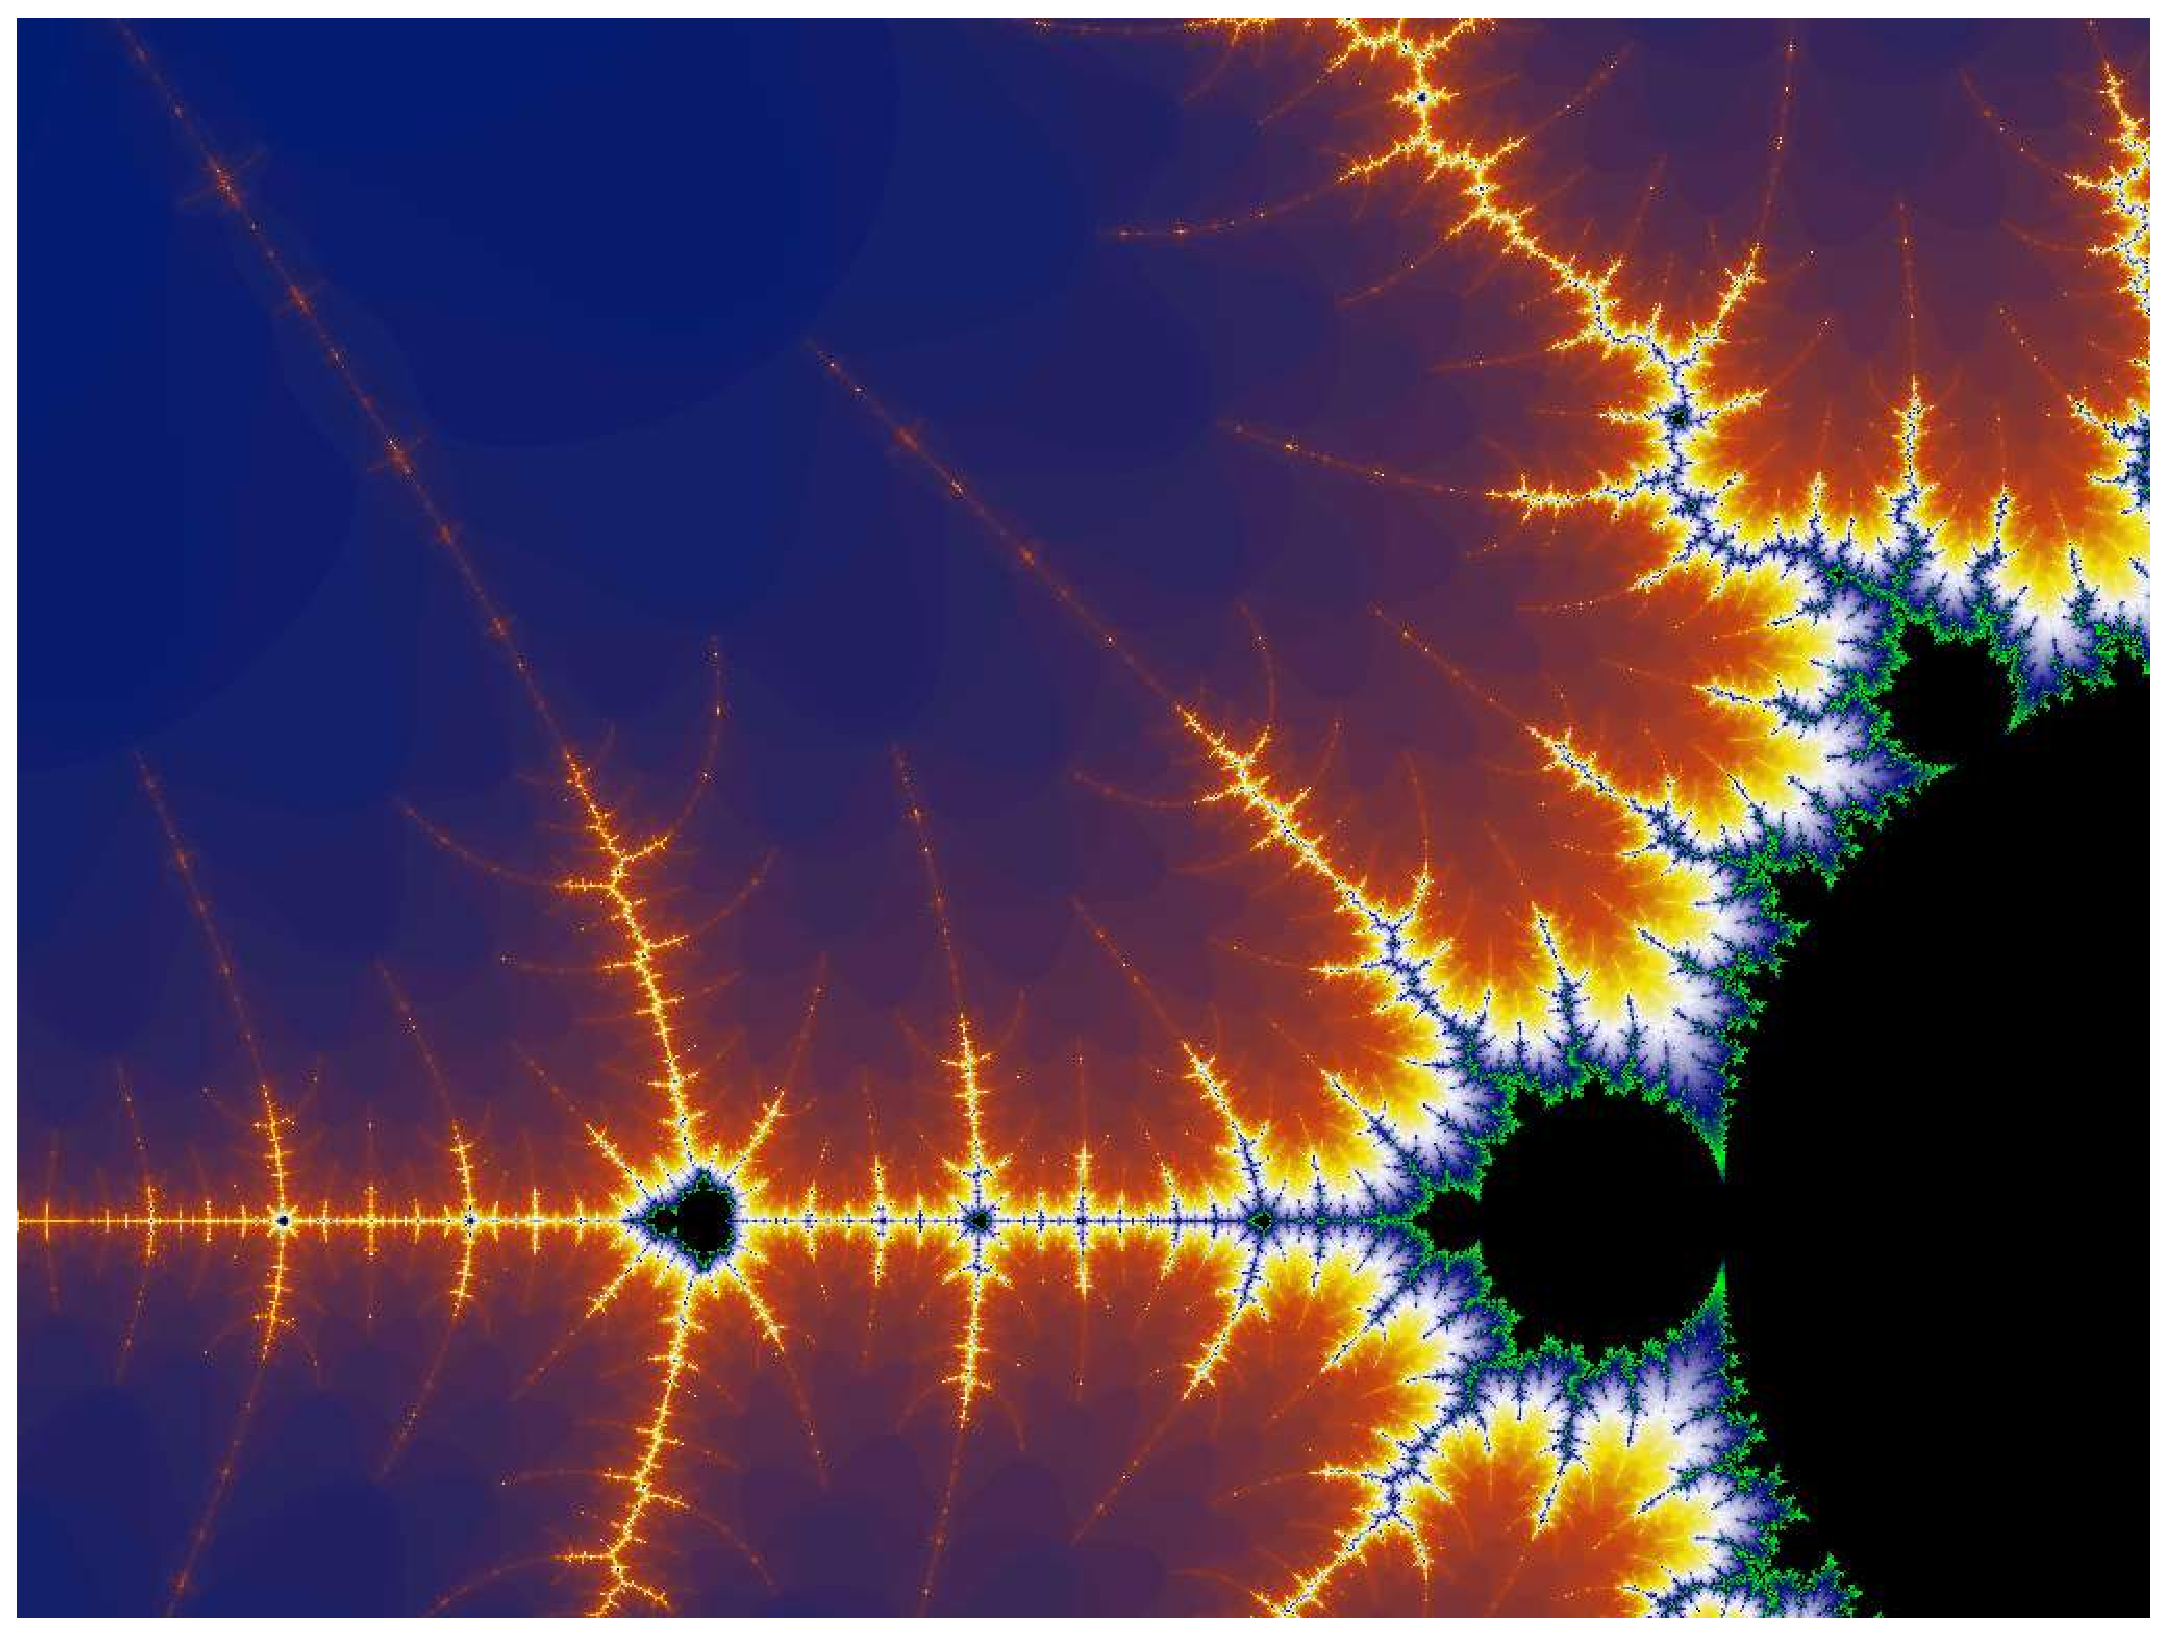
\includegraphics[scale=.2]{mandelbrot}
\caption{Mandelbrot Fractal}
\end{center}
\end{figure}
The word "fractal" often has different connotations for laypeople than mathematicians, where the layperson is more likely to be familiar with fractal art than a mathematical conception. The mathematical concept is difficult to formally define even for mathematicians, but key features can be understood with little mathematical background.
\section{Features}
The feature of "self-similarity", for instance, is easily understood by analogy to zooming in with a lens or other device that zooms in on digital images to uncover finer, previously invisible, new structure. If this is done on fractals, however, no new detail appears; nothing changes and the same pattern repeats over and over, or for some fractals, nearly the same pattern reappears over and over. Self-similarity itself is not necessarily counter-intuitive (e.g., people have pondered self-similarity informally such as in the infinite regress in parallel mirrors or the homunculus, the little man inside the head of the little man inside the head...). 
\section{Application/Usage}
Lorem ipsum dolor sit amet, consectetur adipiscing elit. Morbi urna mauris, sagittis sit amet aliquet ut, facilisis et nibh. Praesent turpis tortor, dignissim ut interdum eu, porttitor ut orci. Curabitur laoreet malesuada fermentum. In posuere, purus eu pulvinar luctus, eros urna tempor magna, eu tincidunt erat eros nec turpis. Vestibulum at semper lacus. Nullam tristique lacus vel nibh porta a vehicula tellus volutpat. Pellentesque cursus ullamcorper ante, ut eleifend nisl aliquam id. Nulla porta ornare fermentum. Aliquam id magna sed erat malesuada viverra. Donec non mauris eros, nec egestas ligula. Suspendisse eu tempor ligula. Aliquam egestas nulla vel augue iaculis iaculis nec in risus. Pellentesque habitant morbi tristique senectus et netus et malesuada fames ac turpis egestas. Praesent malesuada fringilla sapien a faucibus.
\section{Schedule}

\begin{tabular}{|c|c|c|c|}
	\hline Sl No & Date  & No of Hours  & Work done  \\ 
	\hline  &  &  &  \\ 
	\hline  &  &  &  \\ 
	\hline  &  &  &  \\ 
	\hline  &  &  &  \\ 
	\hline 
\end{tabular} 

\chapter{Modules of Training}

The world population is the sum of all humans on Earth. As of today, it is estimated to number 7.004 billion by the United States Census Bureau. The USCB estimates that the world population exceeded 7 billion on March 12, 2012. According to a separate estimate by the United Nations Population Fund, it reached this milestone on October 31, 2011.
\begin{table}[h!]
\begin{center}
\begin{tabular}{|c|c|c|c|}
\hline Rank & Country & Population  & Percentage  \\ 
\hline 1 & China & 1,347,350,000 & 19.24\% \\ 
\hline 2 & India & 1,210,193,422  & 17.28\% \\ 
\hline 3 & United States & 313,269,000 & 4.47\% \\ 
\hline 
\end{tabular}
\caption{World Population Table} 
\end{center}
\end{table}
The world's population is unevenly distributed, with six of Earth's seven continents being permanently inhabited on a large scale. As of 2012, Asia is the most populous continent, with its 4.1 billion inhabitants accounting for over 60\% of the world population. The world's two most-populated countries alone, China and India, constitute about 37\% of the world's population. Africa is the second-most-populated continent, with around 1 billion people, or 15\% of the world's population. Europe's 733 million people make up 11\% of the world's population, while the Latin American and Caribbean regions are home to 589 million (9\%).


\chapter{Daily Diary}


\section{Day 1 (Use exact date here)}

\section{Day 2}

\section{Day 3}

\section{Day 4}

\chapter{Summary}

Compiled languages arelanguages typically processed by compilers, though theoretically any language can be compiled or interpreted. The important ones are:
\begin{itemize}
\item Ada
\item C
\item C++
\item Fortran
\item Java
\end{itemize}



\begin{thebibliography}{1}
\bibitem{nist} K. Scarfone and P. Mell, ``Guide to intrusion detection and prevention systems
(idps),'' \textit{NIST Special Publication}, vol. 800, no. 2007, p. 94, 2007.
\bibitem{knuth} Wikipedia, ``Donald knuth.'' \url{http://en.wikipedia.org/wiki/Donald_Knuth}.
\end{thebibliography}

\begin{appendices}
\chapter{Sample Code}
\begin{lstlisting}[language=c++]
#include <iostream>
using namespace std;
main()
{
	cout << "Hello world \n";
	return 0;
}
\end{lstlisting}
\end{appendices}


\end{document}
